\documentclass[aspectratio=169]{beamer}

% =================================================================
%  Principles of Numerical Control and Coding
%  A beginner-friendly Beamer deck (fully self-contained: all
%  figures / flowcharts / plots drawn with TikZ, so it compiles anywhere).
% =================================================================

% -------------------------------------------------
% Theme and packages
% -------------------------------------------------
\usetheme{Madrid}
\usecolortheme{default}

\usepackage{amsmath}
\usepackage{amssymb}
\usepackage{bm}
\usepackage{listings}
\usepackage{tikz}
\usepackage{array}
\usepackage{booktabs}
\usepackage{tabularx}
\usepackage{ragged2e}
\usepackage{xcolor}

\usetikzlibrary{shapes.geometric, arrows.meta, positioning, calc, fit, backgrounds}

% -------------------------------------------------
% Colour palette
% -------------------------------------------------
\definecolor{cAccent}{RGB}{0,102,153}     % teal-blue accent
\definecolor{cBox}{RGB}{28,31,42}          % dark box
\definecolor{cGreen}{RGB}{34,139,34}
\definecolor{cRed}{RGB}{178,34,34}
\definecolor{cOrange}{RGB}{204,102,0}
\definecolor{cPurple}{RGB}{102,45,145}
\definecolor{cGrayBg}{RGB}{245,246,248}
\definecolor{codebg}{RGB}{248,248,244}
\definecolor{codekw}{RGB}{0,0,180}
\definecolor{codecomment}{RGB}{0,130,0}
\definecolor{codestr}{RGB}{170,55,20}

% Beamer colour tweaks (match a Madrid-style accent)
\setbeamercolor{structure}{fg=cAccent}
\setbeamertemplate{frametitle continuation}{%
	\ifnum\insertcontinuationcount>1\space(cont...)\fi
}
\setbeamertemplate{navigation symbols}{}
\setbeamertemplate{caption}[numbered]

% -------------------------------------------------
% Listings style for C code
% -------------------------------------------------
\lstdefinestyle{cstyle}{
	language=C,
	backgroundcolor=\color{codebg},
	basicstyle=\ttfamily\footnotesize,
	keywordstyle=\color{codekw}\bfseries,
	commentstyle=\color{codecomment}\itshape,
	stringstyle=\color{codestr},
	numbers=none,
	numberstyle=\tiny\color{gray},
	numbersep=8pt,
	showstringspaces=false,
	breaklines=true,
	frame=single,
	rulecolor=\color{gray!50},
	tabsize=2,
	columns=fullflexible,
	keepspaces=true,
	literate={~}{{$\sim$}}1
}
\lstset{style=cstyle}

% Listings style for G-code (ISO 6983 word-address programs)
\lstdefinelanguage{gcode}{
	morekeywords={G00,G01,G02,G03,G17,G21,G28,G40,G41,G42,G80,G81,G90,G91,G94,G98},
	morekeywords=[2]{M03,M05,M06,M08,M09,M30},
	morecomment=[s]{(}{)},
	sensitive=true
}
\lstdefinestyle{gstyle}{
	style=cstyle,
	language=gcode,
	breaklines=false,     % breaklines stops ( ) comments from closing
	keywordstyle=\color{codekw}\bfseries,
	keywordstyle=[2]\color{cRed}\bfseries,
	commentstyle=\color{codecomment}\itshape
}

% Listings style for APT (Automatically Programmed Tools)
\lstdefinelanguage{apt}{
	morekeywords={PARTNO,MACHIN,CLPRNT,UNITS,CUTTER,TOLER,POINT,LINE,CIRCLE,PLANE,
		CENTER,RADIUS,FROM,GO,GOTO,GORGT,GOLFT,GOFWD,GOBACK,GOUP,GODOWN,GODLTA,
		TO,ON,PAST,TANTO,TLRGT,TLLFT,TLON,SPINDL,FEDRAT,COOLNT,CLW,CCLW,FINI,OFF,MM},
	morecomment=[l]{\$\$},
	sensitive=true
}
\lstdefinestyle{aptstyle}{
	style=cstyle,
	language=apt,
	keywordstyle=\color{codekw}\bfseries,
	commentstyle=\color{codecomment}\itshape
}

% Handy TikZ flowchart node styles
\tikzset{
	startstop/.style={rectangle, rounded corners=10pt, minimum width=2.4cm, minimum height=0.8cm, text centered, align=center, draw=black, fill=cAccent!25},
	process/.style  ={rectangle, minimum width=2.6cm, minimum height=0.8cm, text centered, align=center, text width=2.8cm, draw=black, fill=blue!8},
	io/.style       ={trapezium, trapezium left angle=70, trapezium right angle=110, minimum width=2.2cm, minimum height=0.8cm, text centered, align=center, draw=black, fill=cOrange!20},
	decision/.style ={diamond, aspect=2, minimum width=2.4cm, minimum height=0.9cm, text centered, text width=2.2cm, draw=black, fill=cGreen!18, inner sep=1pt},
	flowarrow/.style={-{Stealth[length=2.5mm]}, thick},
	% control-system block diagram styles
	blk/.style      ={rectangle, draw=black, thick, minimum width=1.9cm, minimum height=0.9cm, align=center, fill=blue!8},
	sumj/.style     ={circle, draw=black, thick, minimum size=0.55cm, inner sep=0pt},
	sig/.style      ={-{Stealth[length=2.2mm]}, thick},
}

\setbeamertemplate{footnote}{%
	\parindent 0em
	\noindent
	\raggedright
	\insertfootnotemark\insertfootnotetext\par
}

% -------------------------------------------------
% Title information
% -------------------------------------------------
\title[Principles of NC \& Coding]{Principles of Numerical Control and Coding}
\subtitle{Automation, NC / CNC / DNC, Part Programming, APT \& Economics}
\author[Amit Kumar Singh]{}
\institute[]{
	Amit Kumar Singh \\
	\vspace{0.1cm}
	Assistant Professor (ECE) \\
	\vspace{0.05cm}
	School of Naval Architecture and Ocean Engineering\\
	\vspace{0.05cm}
	Indian Maritime University Visakhapatnam Campus, Sabbavaram Mandal\\
	\vspace{0.05cm}
	Visakhapatnam, Andhra Pradesh -- 531~035\\
	\vspace{0.25cm}
	amitkumarsingh@imu.ac.in
}
\date[AI \& Automation]{\today}

\begin{document}

	%------------------------------------------------
	\begin{frame}
		\titlepage
	\end{frame}

	%------------------------------------------------
	\begin{frame}{Outline}
		\small
		\begin{columns}[T,onlytextwidth]
			\hspace{0.8cm}% shift the first column to the right
			\begin{column}{0.49\textwidth}
				\tableofcontents[hideallsubsections, sections={1-5}]
			\end{column}
			\hspace{0.8cm}% wider gap between the two columns
			\begin{column}{0.40\textwidth}
				\tableofcontents[hideallsubsections, sections={6-9}]
			\end{column}
		\end{columns}
	\end{frame}

	% =================================================================
	\section{Basic Principles of Automation}
	% =================================================================
	\begin{frame}{What is Automation?}
		\begin{block}{Definition}
			\textbf{Automation} is the technology by which a process or procedure is carried out
			with \textbf{minimum human assistance}, using a \textbf{program of instructions}
			combined with a \textbf{control system} that executes those instructions.
		\end{block}
		\vspace{0.2cm}
		\begin{columns}
			\begin{column}{0.55\textwidth}
				\begin{itemize}
					\item Every automated system has \textbf{three} basic elements:
					\begin{enumerate}\small
						\item \textbf{Power} to run the process and the controls.
						\item A \textbf{program of instructions} (what to do, in which order).
						\item A \textbf{control system} that carries out the program.
					\end{enumerate}
					\item In a machine tool the ``program'' is the \emph{part program}
					and the control system is the \emph{NC controller}.
				\end{itemize}
			\end{column}
			\begin{column}{0.45\textwidth}
				\centering
				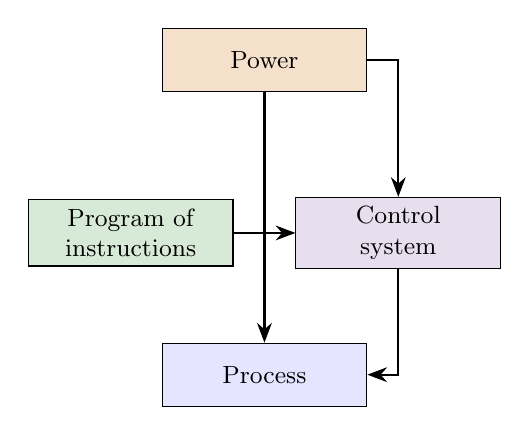
\begin{tikzpicture}[font=\small]
					\node[process, fill=cOrange!20, text width=2.2cm] (pw) at (0,2.2) {Power};
					\node[process, fill=cGreen!18, text width=2.2cm] (pg) at (-1.7,0) {Program of\\ instructions};
					\node[process, fill=cPurple!15, text width=2.2cm] (cs) at (1.7,0) {Control\\ system};
					\node[process, fill=blue!10, text width=2.0cm] (pr) at (0,-1.8) {Process};
					\draw[flowarrow] (pw) -- (pr);
					\draw[flowarrow] (pg) -- (cs);
					\draw[flowarrow] (cs) |- (pr);
					\draw[flowarrow] (pw) -| (cs);
				\end{tikzpicture}
			\end{column}
		\end{columns}
	\end{frame}

	\begin{frame}{Types of Automation}
		\begin{columns}[T]
			\begin{column}{0.32\textwidth}
				\begin{block}{Fixed}
					\centering
					\textbf{Hard automation}

					\vspace{0.2cm}

					\begin{itemize}\small
						\item Sequence fixed by the equipment.
						\item Very high volume, one product.
						\item Low cost per part.
						\item Transfer lines.
					\end{itemize}
				\end{block}
			\end{column}
			\begin{column}{0.32\textwidth}
				\begin{block}{Programmable}
					\centering
					\textbf{Change the program}

					\vspace{0.2cm}

					\begin{itemize}\small
						\item New product = new program.
						\item Batch production, medium volume.
						\item Set-up time lost.
						\item \textbf{NC / CNC}, PLCs.
					\end{itemize}
				\end{block}
			\end{column}
			\begin{column}{0.32\textwidth}
				\begin{block}{Flexible}
					\centering
					\textbf{No lost changeover time}

					\vspace{0.2cm}

					\begin{itemize}\small
						\item Mix of different parts run together.
						\item Set-ups prepared off-line.
						\item Flexible mfg.\ systems (FMS).
					\end{itemize}
				\end{block}
			\end{column}
		\end{columns}
		\vspace{0.1cm}
		\centering
		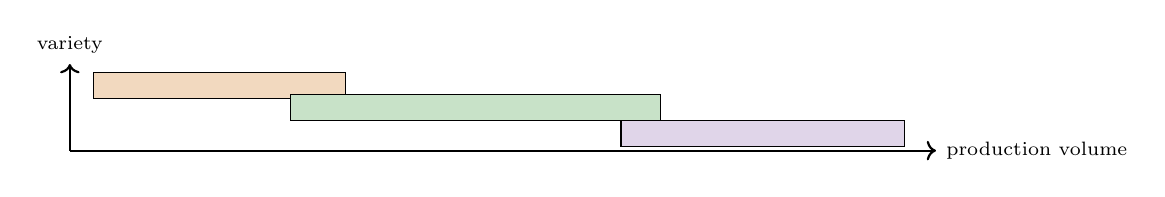
\begin{tikzpicture}[font=\scriptsize, x=1.0cm, y=0.55cm]
			\draw[->, thick] (0,0) -- (11,0) node[right] {production volume};
			\draw[->, thick] (0,0) -- (0,2.0) node[above] {variety};
			\fill[cOrange!25, draw=black] (0.3,1.2) rectangle (3.5,1.8) node[midway] {Manual / conventional};
			\fill[cGreen!25, draw=black] (2.8,0.7) rectangle (7.5,1.3) node[midway] {Programmable (NC, CNC, FMS)};
			\fill[cPurple!20, draw=black] (7.0,0.1) rectangle (10.6,0.7) node[midway] {Fixed automation};
		\end{tikzpicture}
	\end{frame}

	\begin{frame}{Reasons for Automating and the USA Principle}
		\begin{columns}[T]
			\begin{column}{0.5\textwidth}
				\begin{block}{Why automate?}
					\begin{itemize}\small
						\item Increase labour \textbf{productivity}.
						\item Reduce labour cost \& overcome labour shortages.
						\item Remove workers from \textbf{unsafe} or tedious tasks.
						\item Improve \textbf{quality} and consistency.
						\item Reduce manufacturing \textbf{lead time}.
						\item Do what cannot be done manually (complex 3-D shapes).
					\end{itemize}
				\end{block}
			\end{column}
			\begin{column}{0.5\textwidth}
				\begin{block}{The USA principle}
					Before automating any process, follow three steps:
					\begin{enumerate}\small
						\item \textbf{U}nderstand the existing process.
						\item \textbf{S}implify it --- remove unnecessary steps.
						\item \textbf{A}utomate what remains.
					\end{enumerate}
				\end{block}
				\vspace{0.1cm}
				\footnotesize Automating a bad process only makes bad parts \emph{faster}.
			\end{column}
		\end{columns}
	\end{frame}

	\begin{frame}{Ten Strategies for Automation and Process Improvement}
		\renewcommand{\arraystretch}{1.18}
		\centering
		\small
		\begin{tabular}{@{}rp{5.2cm}p{7.0cm}@{}}
			\toprule
			\textbf{\#} & \textbf{Strategy} & \textbf{Example} \\
			\midrule
			1  & Specialisation of operations    & special-purpose tools for one operation \\
			2  & Combined operations              & several cuts in one set-up (machining centre) \\
			3  & Simultaneous operations          & several tools cutting at the same time \\
			4  & Integration of operations        & machines linked by automatic transfer \\
			5  & Increased flexibility            & same machine for many parts (CNC) \\
			6  & Improved material handling       & conveyors, AGVs, automated storage \\
			7  & On-line inspection               & probing the part on the machine \\
			8  & Process control \& optimisation  & adaptive control of feed and speed \\
			9  & Plant operations control         & computer networks, DNC \\
			10 & Computer-integrated manufacturing (CIM) & CAD, CAM, planning in one database \\
			\bottomrule
		\end{tabular}
		\vspace{0.2cm}

		\footnotesize\centering Strategies 2, 5, 7, 8 and 9 are exactly what \textbf{NC, CNC, DNC and adaptive control} provide.
	\end{frame}

	% =================================================================
	\section{Extending Conventional Machines: Devices \& Manipulators}
	% =================================================================
	\begin{frame}{Limitations of Conventional Machine Tools}
		\begin{columns}[T]
			\begin{column}{0.5\textwidth}
				\begin{block}{A conventional lathe or milling machine}
					\small The operator reads the drawing, turns the handwheels, watches the dials and decides every movement.
				\end{block}
				\begin{itemize}\small
					\item Accuracy depends on operator \textbf{skill} and fatigue.
					\item Complex contours are slow or impossible.
					\item Long set-up and idle (non-cutting) time.
					\item Poor repeatability from part to part.
				\end{itemize}
			\end{column}
			\begin{column}{0.5\textwidth}
				\centering
				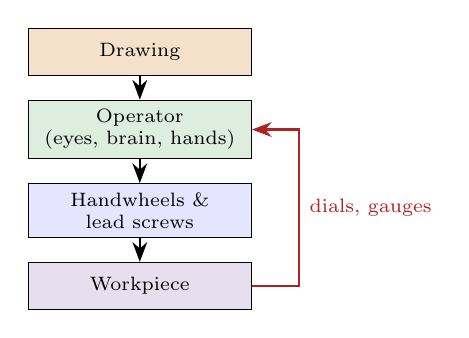
\begin{tikzpicture}[font=\scriptsize, node distance=0.3cm, process/.append style={minimum height=0.6cm}]
					\node[process, fill=cOrange!20, text width=2.6cm] (d) {Drawing};
					\node[process, fill=cGreen!15, below=of d, text width=2.6cm] (o) {Operator\\ (eyes, brain, hands)};
					\node[process, fill=blue!10, below=of o, text width=2.6cm] (m) {Handwheels \&\\ lead screws};
					\node[process, fill=cPurple!15, below=of m, text width=2.6cm] (p) {Workpiece};
					\draw[flowarrow] (d) -- (o);
					\draw[flowarrow] (o) -- (m);
					\draw[flowarrow] (m) -- (p);
					\draw[flowarrow, cRed] (p.east) -- ++(0.6,0) |- node[pos=0.25, right] {dials, gauges} (o.east);
				\end{tikzpicture}
			\end{column}
		\end{columns}
		\vspace{0.1cm}
		\footnotesize\centering The human is the ``control system'' --- the first step is to give the machine devices that take over part of that job.
	\end{frame}

	\begin{frame}{Improved Devices on Conventional Machines}
		\renewcommand{\arraystretch}{1.1}
		\centering
		\footnotesize
		\begin{tabular}{@{}>{\raggedright}p{3.6cm}>{\raggedright}p{5.6cm}>{\raggedright\arraybackslash}p{3.8cm}@{}}
			\toprule
			\textbf{Device} & \textbf{What it does} & \textbf{Benefit} \\
			\midrule
			Power feeds \& rapid traverse & motor drives the slides instead of the operator & less effort, uniform feed \\
			Digital read-out (DRO)        & linear scales display slide position (0.005 mm) & no dial errors or backlash \\
			Copying / tracer attachment  & a stylus follows a template; hydraulics copy it & repeated contours \\
			Turret / capstan head         & several tools pre-set in one indexing head & fast tool change \\
			Cam-operated automatics       & cams sequence every movement & fully automatic, high volume \\
			Jigs, fixtures, quick-change tool posts & locate the part / tool in seconds & short set-up \\
			\bottomrule
		\end{tabular}
		\vspace{0.15cm}
		\begin{block}{Key idea}
			\small Each device automates \emph{one} part of the operator's job. \textbf{Numerical control} automates \emph{all} of it --- the movements come from a program instead of cams or templates.
		\end{block}
	\end{frame}

	\begin{frame}{Manipulators and Industrial Robots}
		\begin{columns}[T]
			\begin{column}{0.55\textwidth}
				\begin{block}{Manipulator}
					A mechanical arm that moves parts or tools. A \textbf{pick-and-place} unit follows a fixed sequence; an \textbf{industrial robot} is a \emph{programmable}, multi-axis manipulator.
				\end{block}
				\begin{itemize}\small
					\item Load / unload machine tools and presses.
					\item Change tools and pallets; transfer parts between machines.
					\item Welding, painting, assembly, inspection.
					\item One robot can serve several CNC machines (a \textbf{cell}).
				\end{itemize}
			\end{column}
			\begin{column}{0.45\textwidth}
				\centering
				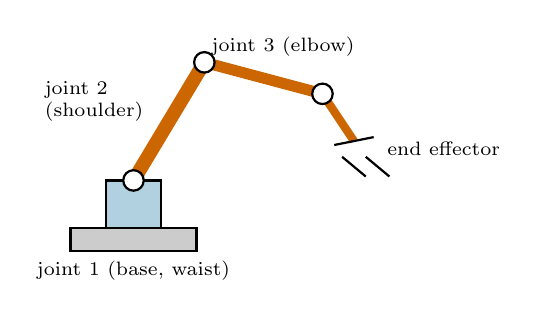
\begin{tikzpicture}[font=\scriptsize]
					% base
					\filldraw[fill=gray!40, thick] (-0.8,0) rectangle (0.8,0.3);
					\filldraw[fill=cAccent!30, thick] (-0.35,0.3) rectangle (0.35,0.9);
					% links
					\draw[line width=5pt, cOrange] (0,0.9) -- (0.9,2.4);
					\draw[line width=4pt, cOrange] (0.9,2.4) -- (2.4,2.0);
					\draw[line width=3pt, cOrange] (2.4,2.0) -- (2.8,1.4);
					% joints
					\foreach \p in {(0,0.9),(0.9,2.4),(2.4,2.0)} \filldraw[fill=white, thick] \p circle (0.13);
					% gripper
					\draw[thick] (2.55,1.35) -- (3.05,1.45);
					\draw[thick] (2.65,1.2) -- (2.95,0.95) (2.95,1.2) -- (3.25,0.95);
					\node[align=left] at (-0.5,1.9) {joint 2\\ (shoulder)};
					\node[align=left] at (1.9,2.6) {joint 3 (elbow)};
					\node[right] at (3.1,1.3) {end effector};
					\node[below] at (0,0) {joint 1 (base, waist)};
				\end{tikzpicture}
				\vspace{0.1cm}

				\footnotesize Articulated arm: 3 arm joints position the wrist; the wrist (2--3 joints) orients the gripper.
			\end{column}
		\end{columns}
	\end{frame}

	\begin{frame}{Robot Configurations and End Effectors}
		\renewcommand{\arraystretch}{1.25}
		\centering
		\small
		\begin{tabular}{@{}lll@{}}
			\toprule
			\textbf{Configuration} & \textbf{Arm joints} & \textbf{Typical use} \\
			\midrule
			Cartesian (gantry)   & L\,L\,L (three linear)                & pick-and-place, CNC loading \\
			Cylindrical          & R\,L\,L (rotate, lift, extend)        & machine loading \\
			Polar (spherical)    & R\,R\,L                               & spot welding, die casting \\
			SCARA                & R\,R\,L (vertical axes)               & fast electronic assembly \\
			Articulated (jointed arm) & R\,R\,R                          & welding, painting, general \\
			\bottomrule
		\end{tabular}
		\vspace{0.3cm}
		\begin{columns}[T]
			\begin{column}{0.5\textwidth}
				\begin{block}{Grippers}
					\small Mechanical fingers, vacuum cups, magnets --- they \emph{hold} the part.
				\end{block}
			\end{column}
			\begin{column}{0.5\textwidth}
				\begin{block}{Tools}
					\small Welding torch, spray gun, spindle, screwdriver --- they \emph{work on} the part.
				\end{block}
			\end{column}
		\end{columns}
		\vspace{0.1cm}
		\footnotesize\centering L = linear (sliding) joint, \; R = rotary joint.
	\end{frame}

	% =================================================================
	\section{Basic Principles of Numerical Control}
	% =================================================================
	\begin{frame}{What is Numerical Control (NC)?}
		\begin{block}{Numerical Control}
			A form of \textbf{programmable automation} in which the mechanical actions of a machine tool
			are controlled by a \textbf{program} of coded \textbf{numbers, letters and symbols}.
		\end{block}
		\vspace{0.1cm}
		\centering
		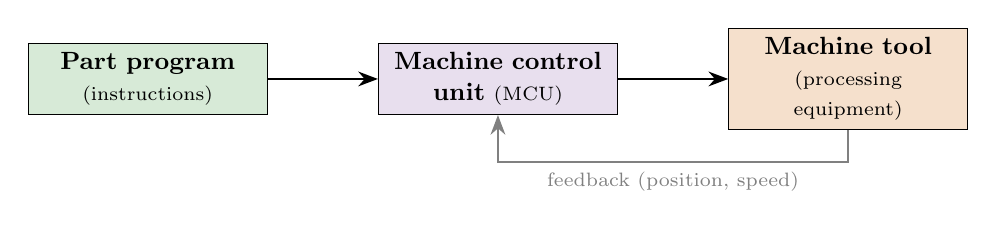
\begin{tikzpicture}[font=\small, node distance=1.4cm]
			\node[process, fill=cGreen!18] (pp) {\textbf{Part program}\\ \scriptsize(instructions)};
			\node[process, right=of pp, fill=cPurple!15] (mcu) {\textbf{Machine control unit} \scriptsize(MCU)};
			\node[process, right=of mcu, fill=cOrange!20] (mt) {\textbf{Machine tool}\\ \scriptsize(processing equipment)};
			\draw[flowarrow] (pp) -- (mcu);
			\draw[flowarrow] (mcu) -- (mt);
			\draw[flowarrow, gray] (mt.south) -- ++(0,-0.4) -| node[pos=0.25, below] {\scriptsize feedback (position, speed)} (mcu.south);
		\end{tikzpicture}
		\vspace{0.1cm}
		\begin{itemize}\small
			\item \textbf{Part program} --- step-by-step instructions: tool positions, feeds, speeds, tool changes, coolant.
			\item \textbf{MCU} --- reads and decodes the program and drives the axes (today: a computer $\rightarrow$ \textbf{CNC}).
			\item \textbf{Machine tool} --- table, spindle, slides, motors that actually cut the metal.
			\item History: J.\,T.\ Parsons \& MIT, first NC milling machine in \textbf{1952} (US Air Force parts).
		\end{itemize}
	\end{frame}

	\begin{frame}{The NC Coordinate System}
		\begin{columns}[T]
			\begin{column}{0.5\textwidth}
				\begin{itemize}\small
					\item Uses the \textbf{right-hand} Cartesian system (ISO 841).
					\item \textbf{Z axis} is always along the \textbf{spindle}; $+Z$ moves the tool \emph{away} from the work.
					\item \textbf{X axis} is the longest horizontal travel; \textbf{Y} completes the right-hand set.
					\item Rotary axes \textbf{A, B, C} rotate about X, Y, Z (5-axis machines).
					\item Positions are measured from the \textbf{program zero} (work datum) chosen by the programmer.
				\end{itemize}
			\end{column}
			\begin{column}{0.5\textwidth}
				\centering
				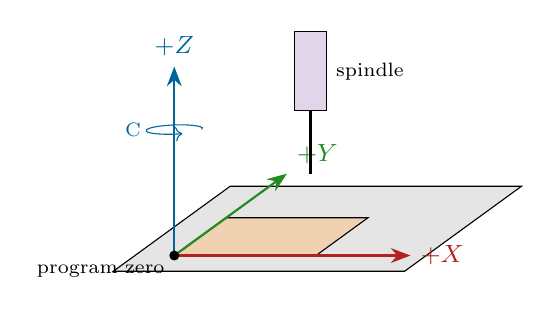
\begin{tikzpicture}[font=\small, x={(1cm,0cm)}, y={(0.55cm,0.4cm)}, z={(0cm,1cm)}]
					% table
					\filldraw[fill=gray!20, draw=black] (-0.5,-0.5,0) -- (3.2,-0.5,0) -- (3.2,2.2,0) -- (-0.5,2.2,0) -- cycle;
					% part
					\filldraw[fill=cOrange!30, draw=black] (0,0,0) -- (1.8,0,0) -- (1.8,1.2,0) -- (0,1.2,0) -- cycle;
					% axes from program zero
					\draw[flowarrow, cRed] (0,0,0) -- (3.0,0,0) node[right] {$+X$};
					\draw[flowarrow, cGreen] (0,0,0) -- (0,2.6,0) node[above right] {$+Y$};
					\draw[flowarrow, cAccent] (0,0,0) -- (0,0,2.4) node[above] {$+Z$};
					\fill (0,0,0) circle (1.8pt) node[below left, font=\scriptsize] {program zero};
					% spindle and tool
					\filldraw[fill=cPurple!20, draw=black] (1.2,0.6,2.6) -- (1.6,0.6,2.6) -- (1.6,0.6,1.6) -- (1.2,0.6,1.6) -- cycle;
					\draw[very thick] (1.4,0.6,1.6) -- (1.4,0.6,0.8);
					\node[right, font=\scriptsize] at (1.6,0.6,2.1) {spindle};
					% rotary C about Z
					\draw[->, cAccent] (0.35,0,1.6) arc (0:300:0.35 and 0.15);
					\node[cAccent, left, font=\scriptsize] at (-0.3,0,1.6) {C};
				\end{tikzpicture}

				\footnotesize Vertical milling machine: tool moves in Z, table moves in X and Y.
			\end{column}
		\end{columns}
	\end{frame}

	\begin{frame}{Point-to-Point vs.\ Continuous-Path (Contouring) Control}
		\begin{columns}[T]
			\begin{column}{0.5\textwidth}
				\begin{block}{Point-to-point (PTP)}
					\small Tool moves to a position \textbf{without cutting}, then the operation is done there. The path between points does not matter.\\
					Drilling, punching, spot welding.
				\end{block}
				\centering
				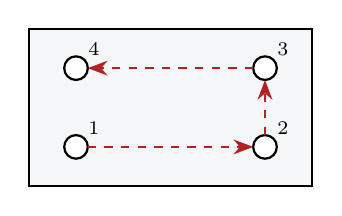
\begin{tikzpicture}[font=\scriptsize]
					\draw[thick, fill=cGrayBg] (0,0) rectangle (3.6,2);
					\foreach \p/\n in {(0.6,0.5)/1,(3.0,0.5)/2,(3.0,1.5)/3,(0.6,1.5)/4}
					\draw[thick, fill=white] \p circle (0.15) node[above right=1pt] {\n};
					\draw[flowarrow, cRed, dashed] (0.75,0.5) -- (2.85,0.5);
					\draw[flowarrow, cRed, dashed] (3.0,0.65) -- (3.0,1.35);
					\draw[flowarrow, cRed, dashed] (2.85,1.5) -- (0.75,1.5);
				\end{tikzpicture}
			\end{column}
			\begin{column}{0.5\textwidth}
				\begin{block}{Continuous path (contouring)}
					\small All axes move \textbf{simultaneously} under control, so the tool follows any line or curve \textbf{while cutting}.\\
					Milling profiles, turning tapers \& radii.
				\end{block}
				\centering
				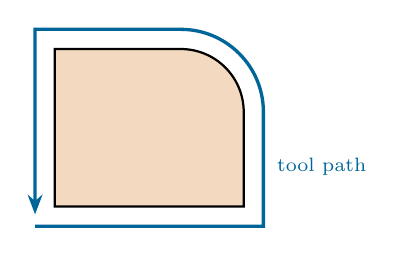
\begin{tikzpicture}[font=\scriptsize]
					\filldraw[thick, fill=cOrange!25] (0,0) -- (2.4,0) -- (2.4,1.2) arc (0:90:0.8) -- (0,2.0) -- cycle;
					\draw[flowarrow, cAccent, very thick] (-0.25,-0.25) -- (2.65,-0.25) -- (2.65,1.2) arc (0:90:1.05) -- (-0.25,2.25) -- (-0.25,-0.1);
					\node[cAccent, right] at (2.7,0.5) {tool path};
				\end{tikzpicture}
			\end{column}
		\end{columns}
		\vspace{0.1cm}
		\footnotesize\centering Contouring needs \textbf{interpolation}: the MCU calculates the intermediate points between the programmed end points.
	\end{frame}

	\begin{frame}{Absolute vs.\ Incremental Positioning}
		\begin{columns}[T]
			\begin{column}{0.45\textwidth}
				\centering
				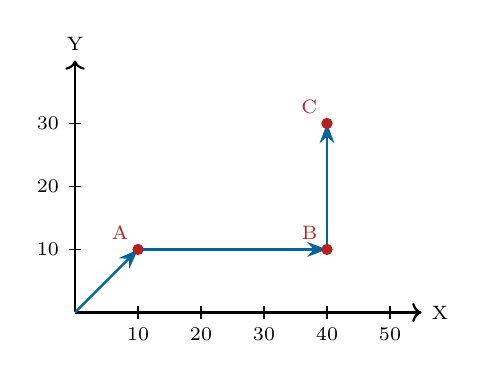
\begin{tikzpicture}[font=\scriptsize, scale=0.08]
					\draw[->, thick] (0,0) -- (55,0) node[right] {X};
					\draw[->, thick] (0,0) -- (0,40) node[above] {Y};
					\foreach \x in {10,20,30,40,50} \draw (\x,1) -- (\x,-1) node[below] {\x};
					\foreach \y in {10,20,30} \draw (1,\y) -- (-1,\y) node[left] {\y};
					\draw[flowarrow, cAccent] (0,0) -- (10,10);
					\draw[flowarrow, cAccent] (10,10) -- (40,10);
					\draw[flowarrow, cAccent] (40,10) -- (40,30);
					\foreach \p/\n in {(10,10)/A,(40,10)/B,(40,30)/C} \fill[cRed] \p circle (0.9) node[above left] {\n};
				\end{tikzpicture}
			\end{column}
			\begin{column}{0.55\textwidth}
				\renewcommand{\arraystretch}{1.3}
				\centering
				\begin{tabular}{@{}lcc@{}}
					\toprule
					\textbf{Move} & \textbf{Absolute (G90)} & \textbf{Incremental (G91)} \\
					\midrule
					0 $\rightarrow$ A & X10 Y10 & X10 Y10 \\
					A $\rightarrow$ B & X40 Y10 & X30 Y0 \\
					B $\rightarrow$ C & X40 Y30 & X0 Y20 \\
					\bottomrule
				\end{tabular}
				\vspace{0.3cm}
				\begin{itemize}\small
					\item \textbf{Absolute}: every position measured from program zero --- an error does not carry forward.
					\item \textbf{Incremental}: each move measured from the \emph{last} position --- handy for repeated patterns.
				\end{itemize}
			\end{column}
		\end{columns}
	\end{frame}

	\begin{frame}{Open-Loop and Closed-Loop NC Systems}
		\vspace*{-0.2cm}
		\begin{block}{Open loop}
			\small The MCU sends a number of \textbf{pulses} to a \textbf{stepper motor}; it assumes the table got there. Cheap, but no correction if steps are missed.
		\end{block}
		\centering
		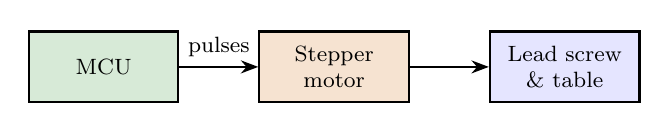
\begin{tikzpicture}[font=\footnotesize, node distance=1.0cm]
			\node[blk, fill=cGreen!18] (c) {MCU};
			\node[blk, right=of c, fill=cOrange!18] (m) {Stepper\\ motor};
			\node[blk, right=of m, fill=blue!10] (s) {Lead screw\\ \& table};
			\draw[sig] (c) -- node[above] {pulses} (m); \draw[sig] (m) -- (s);
		\end{tikzpicture}
		\begin{block}{Closed loop}
			\small A \textbf{servo motor} drives the table and an \textbf{encoder} or linear scale feeds the actual position back; the MCU corrects any error.
		\end{block}
		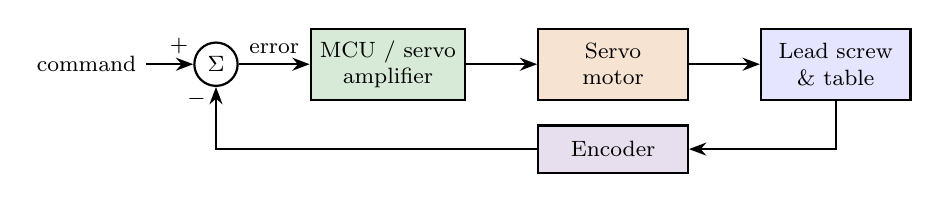
\begin{tikzpicture}[font=\footnotesize, node distance=0.9cm]
			\node (r) {command};
			\node[sumj, right=0.6cm of r] (s) {$\Sigma$};
			\node[blk, right=of s, fill=cGreen!18] (c) {MCU / servo\\ amplifier};
			\node[blk, right=of c, fill=cOrange!18] (m) {Servo\\ motor};
			\node[blk, right=of m, fill=blue!10] (t) {Lead screw\\ \& table};
			\node[blk, below=0.3cm of m, fill=cPurple!15, minimum height=0.6cm] (e) {Encoder};
			\draw[sig] (r) -- node[above, pos=0.7] {$+$} (s);
			\draw[sig] (s) -- node[above] {error} (c);
			\draw[sig] (c) -- (m); \draw[sig] (m) -- (t);
			\draw[sig] (t.south) |- (e);
			\draw[sig] (e) -| node[left, pos=0.9] {$-$} (s);
		\end{tikzpicture}
	\end{frame}

	\begin{frame}{Basic Length Unit (BLU) --- Worked Example}
		\begin{block}{Basic Length Unit}
			The \textbf{smallest} distance the table can be moved by one pulse --- the \textbf{control resolution} of the axis.
			\[
			\text{BLU} = \frac{p}{n_s\, r_g}
			\qquad
			f_p = \frac{v\, r_g\, n_s}{60\,p}
			\]
			$p$ = lead-screw pitch (mm), $n_s$ = steps/rev, $r_g$ = gear ratio (motor : screw), $v$ = feed (mm/min).
		\end{block}
		\begin{columns}[T]
			\begin{column}{0.5\textwidth}
				\textbf{Problem:} open-loop axis, pitch $p = 6$ mm, stepper 200 steps/rev, gear ratio 5:1.
				Find the BLU, the pulses for a 250 mm move, and the pulse rate for a feed of 500 mm/min.
			\end{column}
			\begin{column}{0.5\textwidth}
				\small
				\begin{align*}
					\text{BLU} &= \tfrac{6}{200\times5} = \boxed{0.006\ \text{mm}}\\
					n_p &= \tfrac{250}{0.006} \approx \boxed{41\,667\ \text{pulses}}\\
					f_p &= \tfrac{500\times5\times200}{60\times6} \approx \boxed{1389\ \text{Hz}}
				\end{align*}
			\end{column}
		\end{columns}
	\end{frame}

	\begin{frame}{Precision: Resolution, Accuracy and Repeatability}
		\begin{columns}[T]
			\begin{column}{0.52\textwidth}
				\begin{itemize}\small
					\item \textbf{Control resolution (CR)} --- distance between two adjacent addressable points (= BLU).
					\item \textbf{Accuracy} --- worst-case error in reaching a target:
					\[
					\text{Accuracy} = \frac{\text{CR}}{2} + 3\sigma
					\]
					\item \textbf{Repeatability} --- ability to return to the \emph{same} point: $\pm 3\sigma$.
				\end{itemize}
				\footnotesize $\sigma$ = standard deviation of the mechanical errors (backlash, deflection, thermal).
			\end{column}
			\begin{column}{0.48\textwidth}
				\centering
				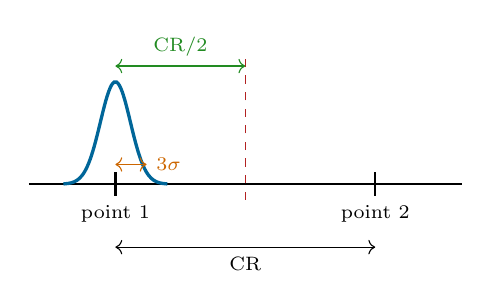
\begin{tikzpicture}[font=\scriptsize, x=1.1cm]
					\draw[thick] (0,0) -- (5,0);
					\foreach \x in {1,4} \draw[thick] (\x,0.15) -- (\x,-0.15);
					\node[below] at (1,-0.15) {point 1};
					\node[below] at (4,-0.15) {point 2};
					\draw[<->] (1,-0.8) -- (4,-0.8) node[midway, below] {CR};
					\draw[dashed, cRed] (2.5,-0.2) -- (2.5,1.6);
					\draw[very thick, cAccent, domain=0.4:1.6, samples=40, smooth] plot (\x, {1.3*exp(-((\x-1)^2)/0.06)});
					\draw[<->, cGreen] (1,1.5) -- (2.5,1.5) node[midway, above] {CR/2};
					\draw[<->, cOrange] (1,0.25) -- (1.36,0.25) node[right] {$3\sigma$};
				\end{tikzpicture}
				\vspace{0.2cm}

				\small \textbf{Example:} CR $= 0.006$ mm, $\sigma = 0.002$ mm\\
				Accuracy $= 0.003 + 0.006 = \boxed{0.009\ \text{mm}}$\\
				Repeatability $= \pm 0.006$ mm
			\end{column}
		\end{columns}
	\end{frame}

	\begin{frame}{Interpolation: Moving Along a Line or Arc}
		\begin{columns}[T]
			\begin{column}{0.55\textwidth}
				\begin{block}{Interpolator}
					\small The part program gives only the \textbf{end points}; the interpolator in the MCU generates the pulse sequence for each axis so the tool stays close to the ideal path.
				\end{block}
				\begin{itemize}\small
					\item \textbf{Linear} (G01) --- straight line in 2 or 3 axes.
					\item \textbf{Circular} (G02 CW / G03 CCW) --- arc in one plane.
					\item Helical, parabolic, spline --- on advanced controls.
					\item The path is really a \textbf{staircase} of BLU steps --- invisible because a BLU is only a few $\mu$m.
				\end{itemize}
			\end{column}
			\begin{column}{0.45\textwidth}
				\centering
				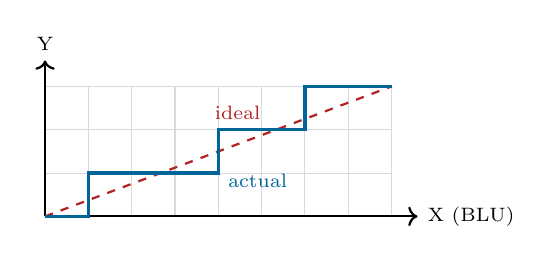
\begin{tikzpicture}[font=\scriptsize, scale=0.55]
					\draw[step=1, gray!30] (0,0) grid (8,3);
					\draw[->, thick] (0,0) -- (8.6,0) node[right] {X (BLU)};
					\draw[->, thick] (0,0) -- (0,3.6) node[above] {Y};
					\draw[thick, dashed, cRed] (0,0) -- (8,3);
					\draw[very thick, cAccent] (0,0) -- (1,0) -- (1,1) -- (2,1) -- (3,1) -- (4,1) -- (4,2) -- (5,2) -- (6,2) -- (6,3) -- (7,3) -- (8,3);
					\node[cRed, above left] at (5.2,2.0) {ideal};
					\node[cAccent, below right] at (4.0,1.2) {actual};
				\end{tikzpicture}

				\footnotesize Line from (0,0) to (8,3) BLU --- the C program later in this deck generates exactly these steps.
			\end{column}
		\end{columns}
	\end{frame}

	% =================================================================
	\section{CNC, DNC and Machining Centres}
	% =================================================================
	\begin{frame}{Computer Numerical Control (CNC)}
		\begin{block}{CNC}
			An NC system whose MCU is a \textbf{dedicated computer}. The part program is stored in memory and executed by software.
		\end{block}
		\begin{columns}[T]
			\begin{column}{0.5\textwidth}
				\begin{block}{Features of CNC}
					\begin{itemize}\small
						\item Program stored, edited \& optimised at the machine.
						\item Interpolation done in software (any type).
						\item Tool-length and cutter-radius compensation.
						\item Canned cycles, sub-programs, macros.
						\item Graphic simulation, diagnostics, communication.
					\end{itemize}
				\end{block}
			\end{column}
			\begin{column}{0.5\textwidth}
				\centering
				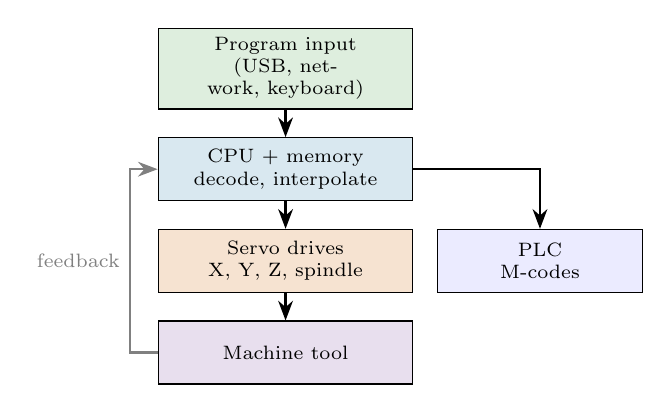
\begin{tikzpicture}[font=\scriptsize, node distance=0.35cm]
					\node[process, fill=cGreen!15, text width=3.0cm] (a) {Program input\\ (USB, network, keyboard)};
					\node[process, fill=cAccent!15, below=of a, text width=3.0cm] (b) {CPU + memory\\ decode, interpolate};
					\node[process, fill=cOrange!18, below=of b, text width=3.0cm] (c) {Servo drives\\ X, Y, Z, spindle};
					\node[process, fill=cPurple!15, below=of c, text width=3.0cm] (d) {Machine tool};
					\node[process, fill=blue!8, right=0.3cm of c, text width=1.3cm] (plc) {PLC\\ M-codes};
					\draw[flowarrow] (a) -- (b); \draw[flowarrow] (b) -- (c); \draw[flowarrow] (c) -- (d);
					\draw[flowarrow] (b.east) -| (plc.north);
					\draw[flowarrow, gray] (d.west) -- ++(-0.35,0) |- node[pos=0.25, left] {feedback} (b.west);
				\end{tikzpicture}
			\end{column}
		\end{columns}
	\end{frame}

	\begin{frame}{How a CNC Executes a Part Program: The Block Cycle}
		\vspace*{-0.3cm}
		\begin{block}{The Read---Decode---Interpolate---Move cycle}
			Just like the CPU's machine cycle, the CNC repeats one cycle for \emph{every} block
			(line) of the part program until it reads \texttt{M30}.
		\end{block}
		\begin{columns}[T]
			\begin{column}{0.55\textwidth}
				\begin{enumerate}\small
					\item \textbf{Read} --- fetch the next block, e.g.\ \texttt{N60 G01 X60 F200}.
					\item \textbf{Decode} --- split it into words: motion type, target, feed, M-codes.
					\item \textbf{Interpolate} --- compute the intermediate points and pulse rates for each axis.
					\item \textbf{Move} --- servo drives move the axes; the PLC handles spindle, coolant, tool change.
					\item \textbf{Check} --- feedback confirms position is reached ``in position'', then go to the next block.
				\end{enumerate}
			\end{column}
			\begin{column}{0.45\textwidth}
				\centering
				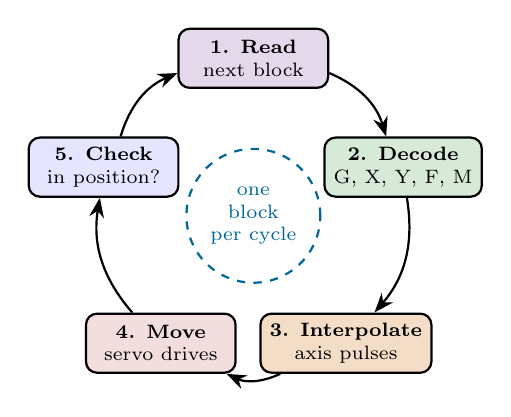
\begin{tikzpicture}[font=\scriptsize,
					stage/.style={rectangle, rounded corners=4pt, draw=black, thick,
						minimum width=1.9cm, minimum height=0.75cm, align=center}]
					\node[circle, draw=cAccent, thick, dashed, minimum size=1.7cm, align=center, text=cAccent]
					(c) at (0,0) {one\\ block\\ per cycle};
					\node[stage, fill=cPurple!18] (r) at (90:2.0)   {\textbf{1. Read}\\ next block};
					\node[stage, fill=cGreen!18]  (d) at (18:2.0)   {\textbf{2. Decode}\\ G, X, Y, F, M};
					\node[stage, fill=cOrange!22] (i) at (-54:2.0)  {\textbf{3. Interpolate}\\ axis pulses};
					\node[stage, fill=cRed!15]    (m) at (-126:2.0) {\textbf{4. Move}\\ servo drives};
					\node[stage, fill=blue!10]    (k) at (162:2.0)  {\textbf{5. Check}\\ in position?};
					\draw[flowarrow] (r) to[bend left=25] (d);
					\draw[flowarrow] (d) to[bend left=25] (i);
					\draw[flowarrow] (i) to[bend left=25] (m);
					\draw[flowarrow] (m) to[bend left=25] (k);
					\draw[flowarrow] (k) to[bend left=25] (r);
				\end{tikzpicture}
			\end{column}
		\end{columns}
	\end{frame}

	\begin{frame}{Direct Numerical Control (DNC)}
		\begin{columns}[T]
			\begin{column}{0.52\textwidth}
				\begin{block}{DNC}
					A \textbf{central computer} stores the part programs and sends them to many machine tools over a network --- originally ``direct'', today \textbf{distributed} NC.
				\end{block}
				\begin{itemize}\small
					\item One library of proven programs --- no lost or outdated tapes.
					\item \textbf{Drip-feeding}: very long 3-D programs streamed block by block.
					\item Collects production data: run time, part count, alarms.
					\item Basis of \textbf{FMS} and computer-integrated manufacturing.
				\end{itemize}
			\end{column}
			\begin{column}{0.48\textwidth}
				\centering
				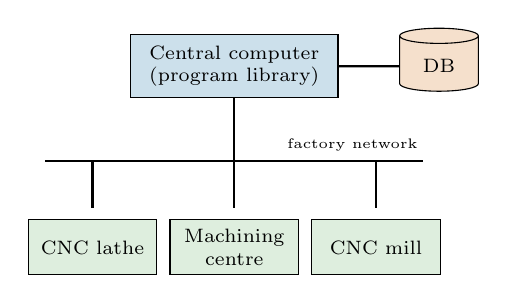
\begin{tikzpicture}[font=\scriptsize]
					\node[process, fill=cAccent!20, text width=2.4cm] (h) at (0,2.4) {Central computer\\ (program library)};
					\node[cylinder, draw=black, shape border rotate=90, aspect=0.3, minimum width=1.0cm, minimum height=0.8cm, fill=cOrange!20] (db) at (2.6,2.4) {DB};
					\draw[thick] (h) -- (db);
					\draw[thick] (-2.4,1.2) -- (2.4,1.2);
					\node[above, font=\tiny] at (1.5,1.2) {factory network};
					\draw[thick] (h) -- (0,1.2);
					\foreach \x/\n in {-1.8/CNC lathe, 0/Machining centre, 1.8/CNC mill} {
						\draw[thick] (\x,1.2) -- (\x,0.6);
						\node[process, fill=cGreen!15, text width=1.4cm, minimum width=1.4cm, minimum height=0.7cm] at (\x,0.1) {\n};
					}
				\end{tikzpicture}
			\end{column}
		\end{columns}
	\end{frame}

	\begin{frame}{Comparing NC, CNC and DNC}
		\renewcommand{\arraystretch}{1.1}
		\centering
		\footnotesize
		\begin{tabular}{@{}>{\raggedright}p{2.6cm}>{\raggedright}p{3.4cm}>{\raggedright}p{3.4cm}>{\raggedright\arraybackslash}p{3.6cm}@{}}
			\toprule
			\textbf{Feature} & \textbf{NC} & \textbf{CNC} & \textbf{DNC} \\
			\midrule
			Controller     & hard-wired logic        & dedicated computer            & central computer + CNCs \\
			Program medium & punched tape, read every part & stored in memory       & stored on server, sent over network \\
			Editing        & punch a new tape        & at the machine                & at the central computer \\
			Interpolation  & hardware                & software                      & software (in each CNC) \\
			Machines       & one                     & one                           & many \\
			Data feedback  & none                    & diagnostics on screen         & production reports \\
			\bottomrule
		\end{tabular}
		\vspace{0.3cm}
		\begin{block}{Key idea}
			\small NC $\rightarrow$ CNC put a computer \emph{in} the machine; CNC $\rightarrow$ DNC connects the machines \emph{to each other}.
		\end{block}
	\end{frame}

	\begin{frame}{Machining Centres}
		\begin{columns}[T]
			\begin{column}{0.55\textwidth}
				\begin{block}{Machining centre}
					A CNC machine tool that performs \textbf{milling, drilling, boring, tapping} on several faces of a part in \textbf{one set-up}, with an \textbf{automatic tool changer}.
				\end{block}
				\begin{itemize}\small
					\item \textbf{ATC} --- tool magazine (20--120 tools) and a change arm; tool change in 1--5 s.
					\item \textbf{APC} --- automatic pallet changer: load the next part while cutting.
					\item \textbf{Types}: vertical (VMC), horizontal (HMC), universal / 5-axis.
					\item \textbf{Turning centre} --- the CNC lathe equivalent, with live tools.
				\end{itemize}
			\end{column}
			\begin{column}{0.45\textwidth}
				\centering
				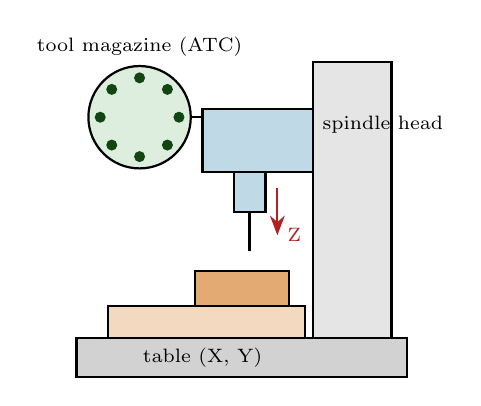
\begin{tikzpicture}[font=\scriptsize]
					% base and column
					\filldraw[fill=gray!35, thick] (0,0) rectangle (4.2,0.5);
					\filldraw[fill=gray!20, thick] (3.0,0.5) rectangle (4.0,4.0);
					% spindle head
					\filldraw[fill=cAccent!25, thick] (1.6,2.6) rectangle (3.0,3.4);
					\filldraw[fill=cAccent!25, thick] (2.0,2.1) rectangle (2.4,2.6);
					\draw[very thick] (2.2,2.1) -- (2.2,1.6);
					% table and part
					\filldraw[fill=cOrange!25, thick] (0.4,0.5) rectangle (2.9,0.9);
					\filldraw[fill=cOrange!55, thick] (1.5,0.9) rectangle (2.7,1.35);
					% tool magazine
					\draw[thick, fill=cGreen!15] (0.8,3.3) circle (0.65);
					\foreach \a in {0,45,...,315} \fill[cGreen!50!black] ($(0.8,3.3)+(\a:0.5)$) circle (0.07);
					\draw[thick] (1.45,3.3) -- (1.6,3.3);
					\node[above] at (0.8,3.95) {tool magazine (ATC)};
					\node[right] at (3.0,3.2) {spindle head};
					\node[below] at (1.6,0.5) {table (X, Y)};
					\draw[flowarrow, cRed] (2.55,2.4) -- (2.55,1.8) node[right] {Z};
				\end{tikzpicture}

				\footnotesize Vertical machining centre (VMC)
			\end{column}
		\end{columns}
	\end{frame}

	% =================================================================
	\section{Methods of Coding}
	% =================================================================
	\begin{frame}{How NC Programs are Stored and Coded}
		\begin{columns}[T]
			\begin{column}{0.5\textwidth}
				\begin{block}{Program input media --- then \& now}
					\begin{itemize}\small
						\item \textbf{Punched tape} (1 inch, 8 tracks) --- the classic NC medium.
						\item Magnetic tape, floppy disk.
						\item Keyboard entry at the CNC (MDI).
						\item USB stick, memory card, Ethernet / DNC.
					\end{itemize}
				\end{block}
				\begin{block}{Two standard character codes}
					\small \textbf{EIA RS-244} --- odd parity, track 5 is the parity track.\\
					\textbf{ISO / ASCII (RS-358)} --- even parity, track 8 is the parity track.
				\end{block}
			\end{column}
			\begin{column}{0.5\textwidth}
				\centering
				\textbf{EIA code for the digits 1--7}\\[4pt]
				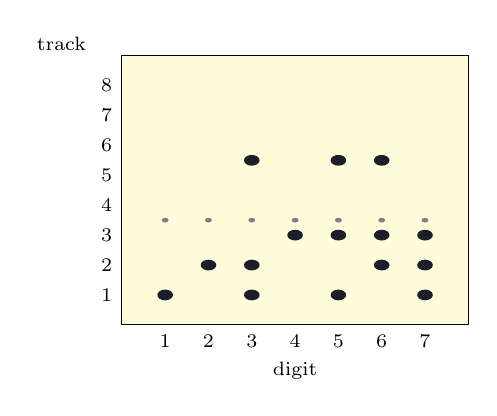
\begin{tikzpicture}[font=\scriptsize, x=0.55cm, y=0.38cm]
					\filldraw[fill=yellow!15, draw=black] (0,0) rectangle (8,9);
					\foreach \t in {1,...,8} \node[left] at (0,{\t+0.5-0.5}) {\t};
					\node[left] at (-0.6,9.4) {track};
					% sprocket holes between track 3 and 4
					\foreach \c in {1,...,7} \fill[gray] (\c,3.5) circle (0.08);
					% digit columns: holes (tracks) incl. EIA parity (track 5)
					\foreach \c/\tr in {1/{1}, 2/{2}, 3/{1,2,5}, 4/{3}, 5/{1,3,5}, 6/{2,3,5}, 7/{1,2,3}} {
						\node[below] at (\c,0) {\c};
						\foreach \t in \tr {
							\pgfmathsetmacro{\yy}{\t<4 ? \t : \t+0.5}
							\fill[cBox] (\c,\yy) circle (0.18);
						}
					}
					\node[below] at (4,-0.9) {digit};
				\end{tikzpicture}

				\footnotesize Tracks 1--4 carry the BCD weights 1, 2, 4, 8. Digit 3 (1+2) has two holes, so track 5 adds a parity hole to make the count \textbf{odd}.
			\end{column}
		\end{columns}
	\end{frame}

	\begin{frame}{Block Formats: Coding an NC Instruction}
		\begin{block}{Block}
			One line of an NC program = one complete instruction (a move plus its conditions).
		\end{block}
		\renewcommand{\arraystretch}{1.15}
		\centering
		\footnotesize
		\begin{tabular}{@{}>{\raggedright}p{2.8cm}>{\raggedright}p{4.6cm}>{\ttfamily\raggedright\arraybackslash}p{5.6cm}@{}}
			\toprule
			\textbf{Format} & \textbf{Rule} & \textrm{\textbf{Example}} \\
			\midrule
			Fixed sequential  & every word, fixed order \& length, no letters & 0050 01 02500 03000 200 \\
			Tab sequential    & fixed order, words separated by TAB; repeated words omitted & 050$\;\to\;$01$\;\to\;$25.0$\;\to\;$30.0 \\
			\textbf{Word address} & each word starts with a \textbf{letter}; any order, only changed words & N050 G01 X25.0 Y30.0 F200 S1000 M03 \\
			\bottomrule
		\end{tabular}
		\vspace{0.15cm}
		\begin{block}{Today}
			\small Every modern CNC uses the \textbf{word-address format} (ISO 6983 ``G-code''). The letter tells the controller what the number means.
		\end{block}
	\end{frame}

	\begin{frame}{Words in a Word-Address Block}
		\renewcommand{\arraystretch}{1.25}
		\centering
		\begin{tabular}{@{}cll@{}}
			\toprule
			\textbf{Letter} & \textbf{Meaning} & \textbf{Example} \\
			\midrule
			\texttt{N} & sequence (block) number             & \texttt{N050} \\
			\texttt{G} & preparatory function (type of motion / mode) & \texttt{G01} linear feed \\
			\texttt{X Y Z} & coordinates of the end point      & \texttt{X25.0 Y30.0} \\
			\texttt{I J K} / \texttt{R} & arc centre offset / radius & \texttt{R10.0} \\
			\texttt{F} & feed rate (mm/min)                   & \texttt{F200} \\
			\texttt{S} & spindle speed (rpm)                  & \texttt{S1000} \\
			\texttt{T} & tool number                          & \texttt{T02} \\
			\texttt{M} & miscellaneous function (on/off)      & \texttt{M03} spindle CW \\
			\bottomrule
		\end{tabular}
		\vspace{0.3cm}

		\centering\small Read a block like a sentence:\;
		\fbox{\texttt{N050 G01 X25.0 Y30.0 F200}} $\rightarrow$ ``step 50: feed in a straight line to (25, 30) at 200 mm/min''.
	\end{frame}

	% =================================================================
	\section{Part Programming}
	% =================================================================
	\begin{frame}{Methods of NC Part Programming}
		\begin{columns}[T]
			\begin{column}{0.32\textwidth}
				\begin{block}{Manual}
					\centering
					\textbf{G-code written by hand}

					\vspace{0.2cm}

					\begin{itemize}\small
						\item Programmer calculates every coordinate.
						\item Best for simple 2-D parts, PTP drilling.
						\item Error-prone for curves.
					\end{itemize}
				\end{block}
			\end{column}
			\begin{column}{0.32\textwidth}
				\begin{block}{Computer-assisted}
					\centering
					\textbf{APT and similar languages}

					\vspace{0.2cm}

					\begin{itemize}\small
						\item Describe geometry \& tool motion in English-like words.
						\item Computer does the maths.
						\item Post-processor makes G-code.
					\end{itemize}
				\end{block}
			\end{column}
			\begin{column}{0.32\textwidth}
				\begin{block}{CAD/CAM \& conversational}
					\centering
					\textbf{Graphical}

					\vspace{0.2cm}

					\begin{itemize}\small
						\item Tool paths generated from the 3-D CAD model.
						\item Simulation before cutting.
						\item Conversational: fill-in screens at the CNC.
					\end{itemize}
				\end{block}
			\end{column}
		\end{columns}
		\vspace{0.3cm}
		\centering
		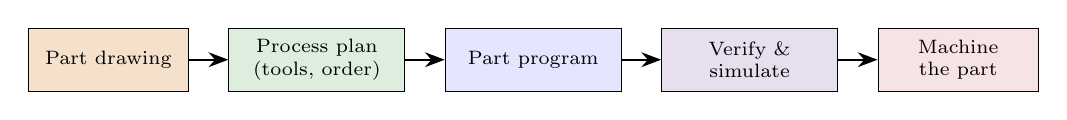
\begin{tikzpicture}[every node/.style={font=\scriptsize}, node distance=0.5cm]
			\node[process, fill=cOrange!20, text width=1.8cm, minimum width=1.8cm] (d) {Part drawing};
			\node[process, right=of d, fill=cGreen!15, text width=2.0cm, minimum width=2.0cm] (pl) {Process plan\\ (tools, order)};
			\node[process, right=of pl, fill=blue!10, text width=2.0cm, minimum width=2.0cm] (pp) {Part program};
			\node[process, right=of pp, fill=cPurple!15, text width=2.0cm, minimum width=2.0cm] (v) {Verify \& simulate};
			\node[process, right=of v, fill=cRed!12, text width=1.8cm, minimum width=1.8cm] (m) {Machine the part};
			\draw[flowarrow] (d) -- (pl); \draw[flowarrow] (pl) -- (pp); \draw[flowarrow] (pp) -- (v); \draw[flowarrow] (v) -- (m);
		\end{tikzpicture}
	\end{frame}

	\begin{frame}{Common G-Codes (Preparatory Functions)}
		\renewcommand{\arraystretch}{1.18}
		\centering
		\small
		\begin{tabular}{@{}cl@{\qquad}cl@{}}
			\toprule
			\textbf{Code} & \textbf{Function} & \textbf{Code} & \textbf{Function} \\
			\midrule
			\texttt{G00} & rapid positioning (no cutting)   & \texttt{G40} & cancel cutter-radius compensation \\
			\texttt{G01} & linear interpolation (feed)      & \texttt{G41} & cutter compensation, tool \textbf{left} \\
			\texttt{G02} & circular interpolation, CW       & \texttt{G42} & cutter compensation, tool \textbf{right} \\
			\texttt{G03} & circular interpolation, CCW      & \texttt{G43} & tool-length compensation \\
			\texttt{G04} & dwell (pause)                    & \texttt{G80} & cancel canned cycle \\
			\texttt{G17} & XY plane selection               & \texttt{G81} & drilling canned cycle \\
			\texttt{G20 / G21} & inch / metric units        & \texttt{G90} & absolute programming \\
			\texttt{G28} & return to reference point        & \texttt{G91} & incremental programming \\
			\bottomrule
		\end{tabular}
		\vspace{0.3cm}
		\begin{block}{Modal codes}
			\small Most G-codes are \textbf{modal}: they stay active until replaced by another code of the same group --- so \texttt{G01} need not be repeated on every line.
		\end{block}
	\end{frame}

	\begin{frame}{Common M-Codes and Cutter-Radius Compensation}
		\begin{columns}[T]
			\begin{column}{0.46\textwidth}
				\renewcommand{\arraystretch}{1.18}
				\centering
				\small
				\begin{tabular}{@{}cl@{}}
					\toprule
					\textbf{Code} & \textbf{Function} \\
					\midrule
					\texttt{M00} & program stop \\
					\texttt{M02} & end of program \\
					\texttt{M03 / M04} & spindle ON, CW / CCW \\
					\texttt{M05} & spindle stop \\
					\texttt{M06} & tool change \\
					\texttt{M08 / M09} & coolant ON / OFF \\
					\texttt{M30} & end of program \& rewind \\
					\bottomrule
				\end{tabular}
			\end{column}
			\begin{column}{0.54\textwidth}
				\begin{block}{Cutter-radius compensation}
					\small The programmer writes the \textbf{part outline}; the CNC offsets the tool centre by the cutter radius.
				\end{block}
				\centering
				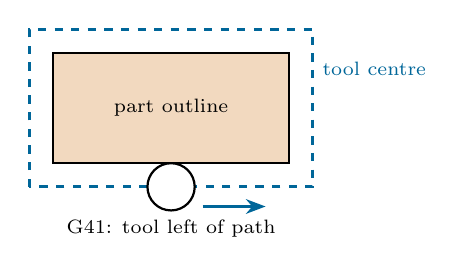
\begin{tikzpicture}[font=\scriptsize]
					\filldraw[fill=cOrange!25, thick] (0,0) rectangle (3,1.4);
					\draw[cAccent, very thick, dashed] (-0.3,-0.3) rectangle (3.3,1.7);
					\draw[thick, fill=white] (1.5,-0.3) circle (0.3);
					\draw[flowarrow, cAccent] (1.9,-0.55) -- (2.7,-0.55);
					\node[below] at (1.5,-0.6) {G41: tool left of path};
					\node at (1.5,0.7) {part outline};
					\node[cAccent, right] at (3.3,1.2) {tool centre};
				\end{tikzpicture}
			\end{column}
		\end{columns}
	\end{frame}

	\begin{frame}[fragile, plain]{}

		\vspace*{0.05cm}

		\begin{columns}[T,onlytextwidth]

			% =========================================================
			% LEFT COLUMN -- PLAN
			% =========================================================

			\begin{column}{0.27\textwidth}

				\begin{block}{Machining plan}
					\scriptsize
					\begin{enumerate}
						\item START; metric, absolute, XY plane
						\item Load tool 1 ($\varnothing$10 end mill)
						\item Rapid above P1, spindle \& coolant ON
						\item Feed down to Z $=-2$
						\item Cut P1 $\to$ P2 $\to$ P3
						\item Arc P3 $\to$ P4 (R10, CCW)
						\item Cut P4 $\to$ P5 $\to$ P1
						\item Retract, coolant \& spindle OFF
						\item STOP (M30)
					\end{enumerate}
				\end{block}

			\end{column}


			% =========================================================
			% MIDDLE COLUMN -- G-CODE PROGRAM
			% =========================================================
			\hspace*{0.3cm}
			\begin{column}{0.42\textwidth}

				\begin{block}{Manual part program (G-code)}

\begin{lstlisting}[style=gstyle,basicstyle=\ttfamily\scriptsize]
O1001 (PROFILE MILLING)
N10 G21 G90 G17
N20 T01 M06        (10 MM END MILL)
N30 G00 X0 Y0 Z5.0
N40 S1200 M03 M08
N50 G01 Z-2.0 F100 (PLUNGE)
N60 X60.0 F200     (P1 TO P2)
N70 Y30.0          (P2 TO P3)
N80 G03 X50.0 Y40.0 R10.0
N90 G01 X0         (P4 TO P5)
N100 Y0            (P5 TO P1)
N110 G00 Z50.0 M09
N120 M05
N130 M30
\end{lstlisting}

				\end{block}

			\end{column}


			% =========================================================
			% RIGHT COLUMN -- PART DRAWING / TOOL PATH
			% =========================================================

			\begin{column}{0.27\textwidth}
				\centering
				\vspace{0.6cm}
				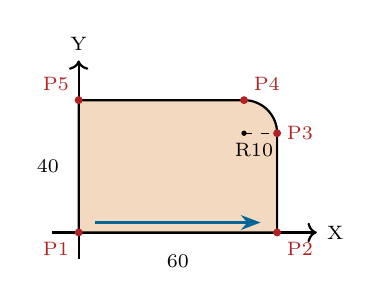
\begin{tikzpicture}[font=\scriptsize, scale=0.042]
					\draw[->, thick] (-8,0) -- (72,0) node[right] {X};
					\draw[->, thick] (0,-8) -- (0,52) node[above] {Y};
					\filldraw[fill=cOrange!25, draw=black, thick] (0,0) -- (60,0) -- (60,30) arc (0:90:10) -- (0,40) -- cycle;
					\draw[flowarrow, cAccent] (5,3) -- (55,3);
					\foreach \p/\n/\pos in {(0,0)/P1/below left, (60,0)/P2/below right, (60,30)/P3/right, (50,40)/P4/above right, (0,40)/P5/above left}
					\fill[cRed] \p circle (1.2) node[\pos] {\n};
					\fill (50,30) circle (0.8);
					\draw[dashed] (50,30) -- (60,30);
					\node[below] at (53,30) {R10};
					\node[below] at (30,-4) {60};
					\node[left] at (-3,20) {40};
				\end{tikzpicture}

				\vspace{0.2cm}
				\scriptsize Program zero at P1 (lower-left corner), top of part = Z0. Tool centre follows the outline (no compensation) for clarity.

			\end{column}

		\end{columns}

	\end{frame}

	\begin{frame}[fragile]{Canned Cycles: Drilling with \texttt{G81}}
		\begin{columns}[T]
			\begin{column}{0.48\textwidth}
\begin{lstlisting}[style=gstyle]
N10 G21 G90 G17
N20 T02 M06        (8 MM DRILL)
N30 S900 M03 M08
N40 G00 X10.0 Y10.0 Z5.0
N50 G81 Z-15.0 R2.0 F80
N60 X50.0          (HOLE 2)
N70 Y30.0          (HOLE 3)
N80 X10.0          (HOLE 4)
N90 G80 G00 Z50.0 M09
N100 M05
N110 M30
\end{lstlisting}
			\end{column}
			\begin{column}{0.52\textwidth}
				\begin{itemize}\small
					\item A \textbf{canned cycle} packs a repeated sequence into one code.
					\item \texttt{G81 Z-15 R2 F80} means: rapid to $R = 2$, feed down to $Z = -15$, rapid back up --- at every new X/Y.
					\item Four holes need only \textbf{one} cycle line plus the hole positions.
					\item \texttt{G80} cancels the cycle.
				\end{itemize}
				\centering
				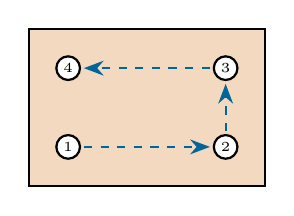
\begin{tikzpicture}[font=\scriptsize, scale=0.05]
					\filldraw[fill=cOrange!25, draw=black, thick] (0,0) rectangle (60,40);
					\foreach \p/\n in {(10,10)/1,(50,10)/2,(50,30)/3,(10,30)/4}
					\draw[thick, fill=white] \p circle (3) node {\tiny\n};
					\draw[flowarrow, cAccent, dashed] (14,10) -- (46,10);
					\draw[flowarrow, cAccent, dashed] (50,14) -- (50,26);
					\draw[flowarrow, cAccent, dashed] (46,30) -- (14,30);
				\end{tikzpicture}
			\end{column}
		\end{columns}
	\end{frame}

	\begin{frame}[fragile, plain]{}

		\vspace*{0.05cm}

		\begin{columns}[T,onlytextwidth]

			% =========================================================
			% LEFT COLUMN -- PSEUDOCODE
			% =========================================================

			\begin{column}{0.25\textwidth}

				\begin{block}{Pseudocode}
					\scriptsize
					\begin{enumerate}
						\item START
						\item READ end point \texttt{dx}, \texttt{dy} (BLU)
						\item \texttt{err = 2dy - dx}
						\item \textbf{FOR} each of the \texttt{dx} steps
						\begin{itemize}\scriptsize
							\item pulse X by 1 BLU
							\item if \texttt{err > 0}: pulse Y, \texttt{err -= 2dx}
							\item \texttt{err += 2dy}
							\item PRINT \texttt{X}, \texttt{Y}
						\end{itemize}
						\item STOP
					\end{enumerate}
				\end{block}

			\end{column}


			% =========================================================
			% MIDDLE COLUMN -- C PROGRAM
			% =========================================================
			\hspace*{0.3cm}
			\begin{column}{0.47\textwidth}

				\begin{block}{C Program (linear interpolator)}

\begin{lstlisting}[style=cstyle,numbers=none,basicstyle=\ttfamily\scriptsize]
#include <stdio.h>

int main(void)
{
	int dx, dy, x = 0, y = 0, err, i;

	printf("End point in BLU (x y): ");
	scanf("%d %d", &dx, &dy); /* dx>=dy>=0 */

	err = 2*dy - dx;          /* decision */
	for (i = 1; i <= dx; i++) {
		x++;                  /* pulse X */
		if (err > 0) {
			y++;              /* pulse Y */
			err -= 2*dx;
		}
		err += 2*dy;
		printf("Step %d : X=%d Y=%d\n",
		       i, x, y);
	}
	return 0;
}
\end{lstlisting}

				\end{block}

			\end{column}


			% =========================================================
			% RIGHT COLUMN -- OUTPUT
			% =========================================================

			\begin{column}{0.24\textwidth}

				\begin{tikzpicture}[remember picture,overlay]

					\node[
					anchor=north east,
					draw,
					rounded corners=2pt,
					fill=white,
					text width=3.4cm,
					align=left,
					inner sep=6pt
					] at ([xshift=-2mm,yshift=-6mm]current page.north east)
					{
						\textbf{Program Output}\\[3pt]
						\ttfamily\scriptsize
						End point in BLU (x y): 8 3\\
						Step 1 : X=1 Y=0\\
						Step 2 : X=2 Y=1\\
						Step 3 : X=3 Y=1\\
						Step 4 : X=4 Y=1\\
						Step 5 : X=5 Y=2\\
						Step 6 : X=6 Y=2\\
						Step 7 : X=7 Y=3\\
						Step 8 : X=8 Y=3
					};

				\end{tikzpicture}

			\end{column}

		\end{columns}

		\begin{tikzpicture}[remember picture,overlay]
			\node[
			anchor=south east,
			draw,
			rounded corners=2pt,
			fill=cGrayBg,
			text width=3.4cm,
			align=left,
			inner sep=6pt,
			font=\scriptsize
			] at ([xshift=-2mm,yshift=4mm]current page.south east)
			{
				\textbf{Note:} these are the steps drawn on the \emph{Interpolation} slide. A real CNC runs this logic thousands of times per second for every axis.
			};
		\end{tikzpicture}

	\end{frame}

	% =================================================================
	\section{APT Programming}
	% =================================================================
	\begin{frame}{APT: Automatically Programmed Tools}
		\begin{block}{APT}
			The first and most widely used \textbf{NC part-programming language}, developed at MIT (1956--59). The programmer describes the \textbf{geometry} and the \textbf{tool motion} in English-like statements; the computer calculates the tool path.
		\end{block}
		\centering
		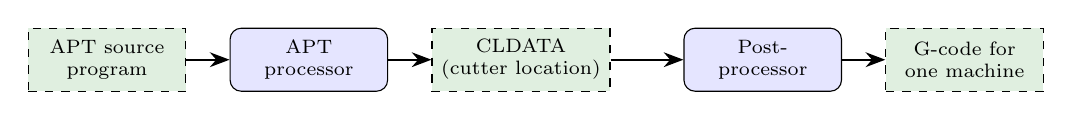
\begin{tikzpicture}[every node/.style={font=\scriptsize}, node distance=0.55cm,
			tool/.style={rectangle, draw=black, rounded corners, minimum width=2.0cm, minimum height=0.8cm, align=center, fill=blue!10},
			art/.style ={rectangle, draw=black, dashed, minimum width=2.0cm, minimum height=0.8cm, align=center, fill=cGreen!14}]
			\node[art] (src) {APT source\\ program};
			\node[tool, right=of src] (proc) {APT\\ processor};
			\node[art, right=of proc] (cl) {CLDATA\\ (cutter location)};
			\node[tool, right=of proc, xshift=3.2cm] (post) {Post-\\ processor};
			\node[art, right=of post] (gc) {G-code for\\ one machine};
			\draw[flowarrow] (src) -- (proc);
			\draw[flowarrow] (proc) -- (cl);
			\draw[flowarrow] (cl) -- (post);
			\draw[flowarrow] (post) -- (gc);
		\end{tikzpicture}
		\vspace{0.2cm}
		\begin{itemize}\small
			\item The \textbf{processor} is machine-independent: it computes the cutter-centre path (CLDATA).
			\item The \textbf{post-processor} converts CLDATA into the codes of a \emph{particular} machine and controller.
			\item Same idea as a C compiler + linker: one source program, many target machines.
		\end{itemize}
	\end{frame}

	\begin{frame}{The Four Types of APT Statements}
		\renewcommand{\arraystretch}{1.3}
		\centering
		\small
		\begin{tabular}{@{}>{\raggedright}p{2.6cm}>{\raggedright}p{4.2cm}>{\ttfamily\raggedright\arraybackslash}p{6.0cm}@{}}
			\toprule
			\textbf{Type} & \textbf{Purpose} & \textrm{\textbf{Examples}} \\
			\midrule
			\textbf{Geometry}  & define points, lines, circles, planes & P1 = POINT/0, 0, 0\newline L1 = LINE/P1, P2\newline C1 = CIRCLE/CENTER, PC, RADIUS, 10 \\
			\textbf{Motion}    & describe the tool path              & FROM/P0 \quad GOTO/P1\newline GORGT/L1, PAST, L2 \\
			\textbf{Post-processor} & speeds, feeds, coolant, machine & SPINDL/1200, CLW\newline FEDRAT/200 \quad COOLNT/ON \\
			\textbf{Auxiliary} & part name, cutter size, tolerance, end & PARTNO \quad CUTTER/10\newline TOLER/0.01 \quad FINI \\
			\bottomrule
		\end{tabular}
		\vspace{0.3cm}

		\footnotesize\centering Each statement: \texttt{MAJOR WORD / minor words, values}. \; Comments start with \texttt{\$\$}.
	\end{frame}

	\begin{frame}{APT Motion Statements}
		\begin{columns}[T]
			\begin{column}{0.5\textwidth}
				\begin{block}{Point-to-point}
					\small \texttt{FROM/P0} --- starting point\\
					\texttt{GOTO/P1} --- go to an absolute point\\
					\texttt{GODLTA/20, 0, -5} --- incremental move
				\end{block}
				\begin{block}{Contouring --- direction words}
					\small \texttt{GOLFT} / \texttt{GORGT} --- turn left / right\\
					\texttt{GOFWD} / \texttt{GOBACK} --- go forward / back\\
					\texttt{GOUP} / \texttt{GODOWN} --- up / down
				\end{block}
			\end{column}
			\begin{column}{0.5\textwidth}
				\begin{block}{Where the tool stops (check surface)}
					\small \texttt{TO} --- tool just touches it\\
					\texttt{ON} --- tool centre on it\\
					\texttt{PAST} --- tool just beyond it\\
					\texttt{TANTO} --- tangent point of a curve
				\end{block}
				\centering
				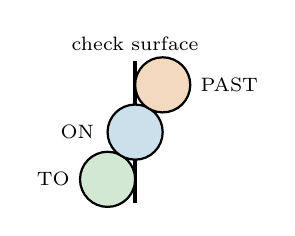
\begin{tikzpicture}[font=\scriptsize]
					\draw[very thick] (0,0) -- (0,1.8) node[above] {check surface};
					\draw[thick, fill=cGreen!20] (-0.35,0.3) circle (0.35) node[left=0.35cm] {TO};
					\draw[thick, fill=cAccent!20] (0,0.9) circle (0.35);
					\node[left] at (-0.4,0.9) {ON};
					\draw[thick, fill=cOrange!25] (0.35,1.5) circle (0.35) node[right=0.35cm] {PAST};
				\end{tikzpicture}
			\end{column}
		\end{columns}
		\vspace{0.1cm}
		\footnotesize\centering Tool position relative to the drive surface: \texttt{TLLFT}, \texttt{TLRGT} (left / right of it) or \texttt{TLON} (on it).
	\end{frame}

	\begin{frame}[fragile, plain]{}

		\vspace*{0.05cm}

		\begin{columns}[T,onlytextwidth]

			% =========================================================
			% LEFT COLUMN -- APT GEOMETRY
			% =========================================================
			
			\begin{column}{0.34\textwidth}
				
				\begin{block}{APT (1): set-up \& geometry}
					
\begin{lstlisting}[style=aptstyle,basicstyle=\ttfamily\scriptsize]
PARTNO PROFILE MILLING
MACHIN/MILL, 1
UNITS/MM
CUTTER/10.0
TOLER/0.01
$$ ----- geometry -----
P0 = POINT/-20, -20, 10
P1 = POINT/0, 0, 0
P2 = POINT/60, 0, 0
P3 = POINT/60, 30, 0
P5 = POINT/50, 40, 0
P6 = POINT/0, 40, 0
PC = POINT/50, 30, 0
L1 = LINE/P1, P2
L2 = LINE/P2, P3
C1 = CIRCLE/CENTER, PC, $
     RADIUS, 10
L3 = LINE/P5, P6
L4 = LINE/P6, P1
PL1 = PLANE/0, 0, 1, -2
\end{lstlisting}
					
				\end{block}
				
			\end{column}
			
			
			% =========================================================
			% MIDDLE COLUMN -- APT MOTION
			% =========================================================
			
			\begin{column}{0.33\textwidth}
				
				\begin{block}{APT (2): motion}
					
\begin{lstlisting}[style=aptstyle,basicstyle=\ttfamily\scriptsize]
$$ ----- machining -----
SPINDL/1200, CLW
FEDRAT/200
COOLNT/ON
FROM/P0
GO/TO, L1, TO, PL1, TO, L4
TLRGT, GORGT/L1, PAST, L2
GOLFT/L2, TANTO, C1
GOFWD/C1, TANTO, L3
GOFWD/L3, PAST, L4
GOLFT/L4, PAST, L1
GOTO/P0
COOLNT/OFF
SPINDL/OFF
FINI
\end{lstlisting}
					
				\end{block}
				
				\footnotesize A single \texttt{\$} at the end of a line continues the statement on the next line.
				
			\end{column}
			
			
			% =========================================================
			% RIGHT COLUMN -- GEOMETRY
			% =========================================================
			
			\begin{column}{0.31\textwidth}
				\centering
				\vspace{0.7cm}
				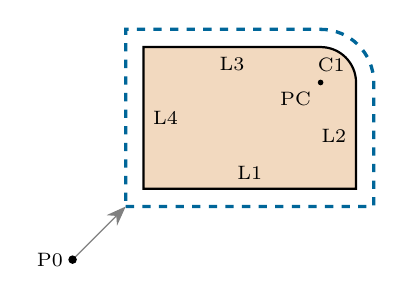
\begin{tikzpicture}[font=\scriptsize, scale=0.045]
					\filldraw[fill=cOrange!25, draw=black, thick] (0,0) -- (60,0) -- (60,30) arc (0:90:10) -- (0,40) -- cycle;
					% tool-centre path (offset by cutter radius 5)
					\draw[cAccent, very thick, dashed] (-5,-5) -- (65,-5) -- (65,30) arc (0:90:15) -- (-5,45) -- (-5,-5);
					\draw[flowarrow, thin, gray] (-20,-20) -- (-5,-5);
					\fill (-20,-20) circle (1.2) node[left] {P0};
					\node[above] at (30,0) {L1};
					\node[left] at (60,15) {L2};
					\node at (53,35) {C1};
					\node[below] at (25,40) {L3};
					\node[right] at (0,20) {L4};
					\fill (50,30) circle (0.8) node[below left] {PC};
				\end{tikzpicture}
				
				\scriptsize\textcolor{cAccent}{dashed} = tool-centre path
				
				\vspace{0.1cm}
				\begin{block}{Reading the motion}
					\scriptsize
					\texttt{GO/TO, L1, TO, PL1, TO, L4} --- touch L1 and L4 at depth PL1.\\
					\texttt{TLRGT} --- tool on the right of the drive line (outside).\\
					\texttt{PAST} --- outside corner; \texttt{TANTO} --- change surface at the tangent point.
				\end{block}
				
			\end{column}
			
		\end{columns}

	\end{frame}

	\begin{frame}{Manual Programming vs.\ APT}
		\renewcommand{\arraystretch}{1.3}
		\centering
		\small
		\begin{tabular}{@{}>{\raggedright}p{3.0cm}>{\raggedright}p{4.6cm}>{\raggedright\arraybackslash}p{4.6cm}@{}}
			\toprule
			\textbf{Aspect} & \textbf{Manual (G-code)} & \textbf{APT} \\
			\midrule
			Calculations    & by the programmer (tangent points, offsets) & by the computer \\
			Language        & numbers and codes          & English-like words \\
			Machine-specific & yes                       & no --- post-processor adapts it \\
			Cutter offset   & calculated or G41/G42      & automatic from \texttt{CUTTER/} \\
			Best for        & simple 2-D, drilling       & complex contours, 3- to 5-axis \\
			\bottomrule
		\end{tabular}
		\vspace{0.3cm}
		\begin{block}{Key idea}
			\small APT introduced the ideas that CAD/CAM systems still use today: geometry first, then tool motion, then a post-processor for each machine.
		\end{block}
	\end{frame}

	% =================================================================
	\section{Adaptive Control}
	% =================================================================
	\begin{frame}{What is Adaptive Control?}
		\begin{block}{Adaptive control (AC)}
			A control system that \textbf{measures} process variables during machining (force, torque, power, temperature, vibration) and \textbf{automatically adjusts} feed and speed to suit the actual cutting conditions.
		\end{block}
		\centering
		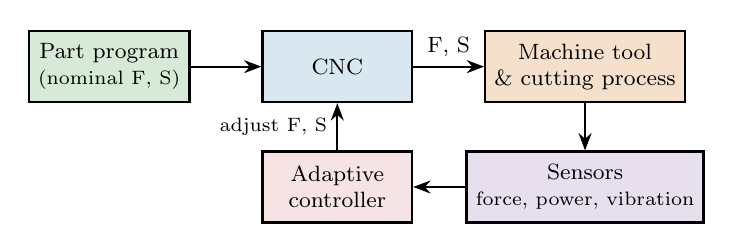
\begin{tikzpicture}[font=\footnotesize, node distance=0.9cm]
			\node[blk, fill=cGreen!18] (p) {Part program\\ \scriptsize(nominal F, S)};
			\node[blk, right=of p, fill=cAccent!15] (cnc) {CNC};
			\node[blk, right=of cnc, fill=cOrange!20] (mt) {Machine tool\\ \& cutting process};
			\node[blk, below=0.6cm of mt, fill=cPurple!15] (sen) {Sensors\\ \scriptsize force, power, vibration};
			\node[blk, below=0.6cm of cnc, fill=cRed!12] (ac) {Adaptive\\ controller};
			\draw[sig] (p) -- (cnc);
			\draw[sig] (cnc) -- node[above] {F, S} (mt);
			\draw[sig] (mt) -- (sen);
			\draw[sig] (sen) -- (ac);
			\draw[sig] (ac) -- node[left] {\scriptsize adjust F, S} (cnc);
		\end{tikzpicture}
		\vspace{0.15cm}
		\begin{itemize}\small
			\item Ordinary NC uses the programmed feed even if the depth of cut or hardness changes.
			\item The programmer must choose \emph{safe} (slow) values for the worst case --- AC removes that penalty.
		\end{itemize}
	\end{frame}

	\begin{frame}{Types of Adaptive Control}
		\begin{columns}[T]
			\begin{column}{0.32\textwidth}
				\begin{block}{ACC --- Constraint}
					\begin{itemize}\small
						\item Keep a variable (force, power) \textbf{at or below a limit}.
						\item Feed increased in light cuts, reduced in heavy cuts.
						\item Most common in practice.
					\end{itemize}
				\end{block}
			\end{column}
			\begin{column}{0.32\textwidth}
				\begin{block}{ACO --- Optimisation}
					\begin{itemize}\small
						\item Maximise a \textbf{performance index} --- e.g.\ metal-removal rate per cost.
						\item Needs on-line tool-wear sensing.
						\item Mostly research systems.
					\end{itemize}
				\end{block}
			\end{column}
			\begin{column}{0.32\textwidth}
				\begin{block}{GAC --- Geometric}
					\begin{itemize}\small
						\item Measure the part (probe) and correct for tool wear \& deflection.
						\item Used in finishing cuts.
						\item Improves \textbf{accuracy}.
					\end{itemize}
				\end{block}
			\end{column}
		\end{columns}
		\vspace{0.3cm}
		\begin{block}{Benefits}
			\small Higher metal-removal rate, fewer broken tools, protection of spindle and part, less programmer effort (no need to guess conservative feeds), consistent quality.
		\end{block}
	\end{frame}

	\begin{frame}{Adaptive Control Constraint: Worked Example}
		\begin{columns}[T]
			\begin{column}{0.5\textwidth}
				\textbf{Problem:} In a milling cut the cutting force is approximately
				\[
				F_c = k\, d\, f
				\]
				($d$ = depth of cut, $f$ = feed per tooth). With $d = 2$ mm and $f = 0.3$ mm the force equals the limit $F_{\max} = 1500$ N. The depth suddenly rises to $3$ mm. What feed must the ACC system select?
			\end{column}
			\begin{column}{0.5\textwidth}
				\textbf{Solution:}
				\small
				\begin{align*}
					k &= \frac{1500}{2\times0.3} = 2500\ \text{N/mm}^2\\
					F_c\ (\text{no AC}) &= 2500\times3\times0.3 = 2250\ \text{N}\ (\text{overload!})\\
					f_{\text{new}} &= \frac{1500}{2500\times3} = \boxed{0.2\ \text{mm}}
				\end{align*}
				\footnotesize When the cut becomes lighter again, the ACC raises the feed back up --- the force stays at the limit all the time.
			\end{column}
		\end{columns}
	\end{frame}

	% =================================================================
	\section{Economics of Numerical Control}
	% =================================================================
	\begin{frame}{Advantages and Disadvantages of NC}
		\begin{columns}[T]
			\begin{column}{0.5\textwidth}
				\begin{block}{Advantages}
					\begin{itemize}\small
						\item Less non-productive time (set-up, handling, measuring).
						\item Greater accuracy \& repeatability, less scrap.
						\item Complex shapes are possible.
						\item Fewer jigs \& fixtures, smaller inventory.
						\item Quick design changes (edit the program).
						\item Shorter manufacturing lead time.
					\end{itemize}
				\end{block}
			\end{column}
			\begin{column}{0.5\textwidth}
				\begin{block}{Disadvantages}
					\begin{itemize}\small
						\item High investment cost.
						\item Higher maintenance effort \& skilled technicians.
						\item Part programming effort and training.
						\item Higher machine-hour rate --- needs high utilisation (2--3 shifts).
					\end{itemize}
				\end{block}
			\end{column}
		\end{columns}
	\end{frame}

	\begin{frame}{Where NC Pays: Cost vs.\ Batch Size}
		\begin{columns}[T]
			\begin{column}{0.55\textwidth}
				\centering
				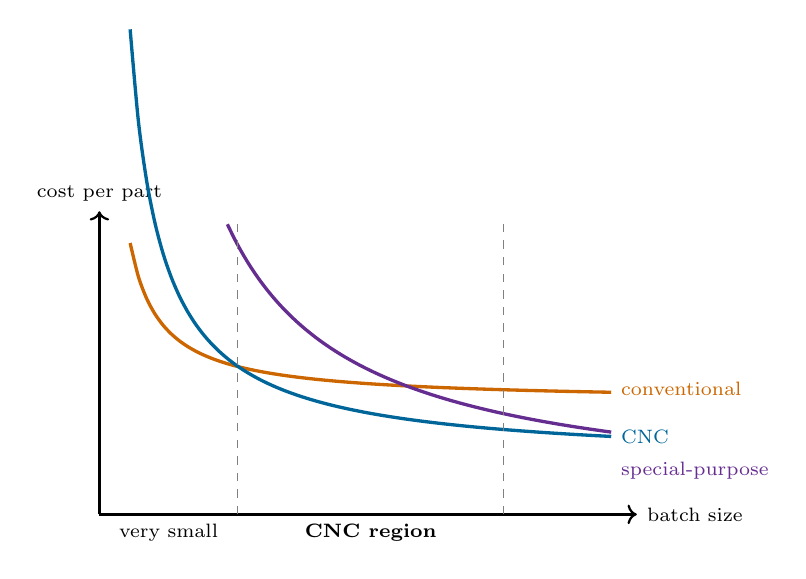
\begin{tikzpicture}[font=\scriptsize, x=0.65cm, y=0.55cm]
					\draw[->, thick] (0,0) -- (10.5,0) node[right] {batch size};
					\draw[->, thick] (0,0) -- (0,7) node[above] {cost per part};
					\draw[very thick, cOrange, domain=0.6:10, samples=60, smooth] plot (\x, {2.6 + 2.2/\x});
					\draw[very thick, cAccent, domain=0.6:10, samples=60, smooth] plot (\x, {1.2 + 6.0/\x});
					\draw[very thick, cPurple, domain=2.5:10, samples=60, smooth] plot (\x, {0.3 + 16/\x});
					\node[cOrange, right] at (10,2.9) {conventional};
					\node[cAccent, right] at (10,1.8) {CNC};
					\node[cPurple, right] at (10,1.0) {special-purpose};
					\draw[dashed, gray] (2.7,0) -- (2.7,6.8);
					\draw[dashed, gray] (7.9,0) -- (7.9,6.8);
					\node[below, text width=1.6cm, align=center] at (1.35,0) {very small};
					\node[below] at (5.3,0) {\textbf{CNC region}};
				\end{tikzpicture}
			\end{column}
			\begin{column}{0.45\textwidth}
				\begin{itemize}\small
					\item \textbf{Very small batches} --- programming \& set-up dominate; conventional machines can be cheaper.
					\item \textbf{Medium batches, many part types} --- CNC is cheapest.
					\item \textbf{Very large volumes of one part} --- special-purpose / transfer machines win.
				\end{itemize}
				\vspace{0.2cm}
				\footnotesize Rising part complexity pushes the CNC region to \emph{smaller} batches.
			\end{column}
		\end{columns}
	\end{frame}

	\begin{frame}{Cost Elements and Justification Methods}
		\begin{columns}[T]
			\begin{column}{0.5\textwidth}
				\begin{block}{Fixed (investment) costs}
					\small Machine \& controller, installation, tooling, software (CAM), training.
				\end{block}
				\begin{block}{Operating costs}
					\small Operator labour, programming, maintenance, power, tool wear, overheads --- usually combined into a \textbf{machine-hour rate}.
				\end{block}
			\end{column}
			\begin{column}{0.5\textwidth}
				\begin{block}{Justification methods}
					\small
					\textbf{Payback period} $= \dfrac{\text{investment}}{\text{net annual saving}}$\\[4pt]
					\textbf{Break-even quantity}: batch size where both methods cost the same.\\[4pt]
					\textbf{Return on investment} / net present value (for larger projects).
				\end{block}
				\vspace{0.1cm}
				\footnotesize \textbf{Example:} a CNC costs Rs 40 lakh and saves Rs 10 lakh per year $\Rightarrow$ payback $= 40/10 = \boxed{4\ \text{years}}$.
			\end{column}
		\end{columns}
	\end{frame}

	\begin{frame}{Break-Even Analysis: Worked Example}
		\begin{columns}[T]
			\begin{column}{0.52\textwidth}
				\renewcommand{\arraystretch}{1.2}
				\centering
				\small
				\begin{tabular}{@{}lcc@{}}
					\toprule
					& \textbf{Conventional} & \textbf{CNC} \\
					\midrule
					Machine-hour rate & Rs 400/h & Rs 1200/h \\
					Set-up per batch  & 4 h      & 1 h \\
					Programming / batch & ---    & Rs 3000 \\
					Cycle time / part & 30 min   & 8 min \\
					\bottomrule
				\end{tabular}
				\vspace{0.1cm}
				\footnotesize
				\begin{align*}
					C_{\text{conv}} &= 400\,(4 + 0.5\,Q) = 1600 + 200\,Q\\
					C_{\text{CNC}} &= 3000 + 1200\,(1 + \tfrac{8}{60}Q) = 4200 + 160\,Q\\
					1600 + 200\,Q &= 4200 + 160\,Q \;\Rightarrow\; \boxed{Q = 65\ \text{parts}}
				\end{align*}
			\end{column}
			\begin{column}{0.48\textwidth}
				\centering
				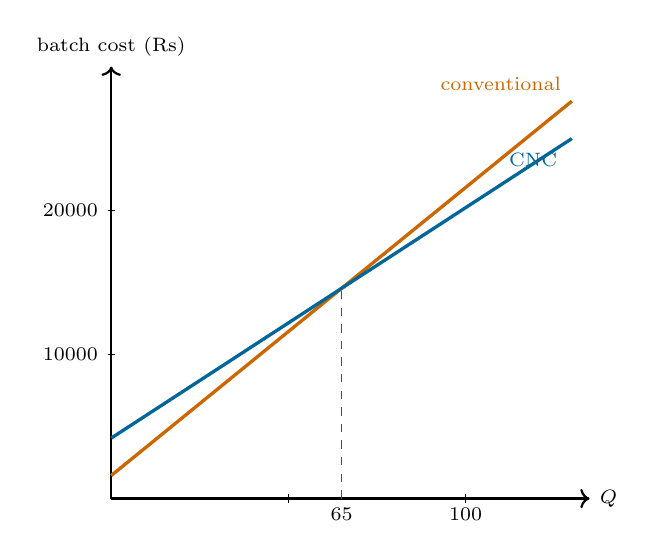
\begin{tikzpicture}[font=\scriptsize, x=0.045cm, y=0.00018cm]
					\draw[->, thick] (0,0) -- (135,0) node[right] {$Q$};
					\draw[->, thick] (0,0) -- (0,30000) node[above] {batch cost (Rs)};
					\draw[very thick, cOrange] (0,1600) -- (130,27600) node[above left] {conventional};
					\draw[very thick, cAccent] (0,4200) -- (130,25000) node[below left=2pt] {CNC};
					\draw[dashed, cRed] (65,0) -- (65,14600);
					\fill[cRed] (65,14600) circle (1.2);
					\node[below] at (65,0) {65};
					\foreach \q in {50,100} \draw (\q,300) -- (\q,-300);
					\node[below] at (100,0) {100};
					\foreach \c in {10000,20000} \draw (1,\c) -- (-1,\c) node[left] {\c};
				\end{tikzpicture}

				\footnotesize Batches \textbf{above 65} parts are cheaper on the CNC; smaller batches on the conventional machine.
			\end{column}
		\end{columns}
	\end{frame}

	\begin{frame}{Summary \& What Comes Next}
		\begin{columns}[T]
			\begin{column}{0.5\textwidth}
				\begin{block}{Concept}
					\begin{itemize}\small
						\item Automation: elements, types, USA principle, 10 strategies.
						\item Improved devices \& manipulators on conventional machines.
						\item NC principles: axes, PTP / contouring, open / closed loop, BLU, interpolation.
						\item CNC, DNC and machining centres.
						\item Coding: tape codes, block formats, G- \& M-codes.
						\item APT programming, adaptive control, economics.
					\end{itemize}
				\end{block}
			\end{column}
			\begin{column}{0.5\textwidth}
				\begin{block}{Practice makes perfect}
					\begin{itemize}\small
						\item Write G-code for a new part and check it in a free simulator.
						\item Re-work the BLU, ACC and break-even examples with new numbers.
						\item Run the interpolation C program for other end points.
					\end{itemize}
				\end{block}
				\begin{block}{Coming up}
					\small CAD/CAM, industrial robotics and flexible manufacturing systems.
				\end{block}
			\end{column}
		\end{columns}
	\end{frame}

	%------------------------------------------------
	\begin{frame}
		\centering
		\Huge Thank You
		\vspace{0.5cm}

		\normalsize Questions?
	\end{frame}

	%------------------------------------------------

\end{document}
